\documentclass[conference]{IEEEtran}
\IEEEoverridecommandlockouts
\usepackage{cite}
\usepackage{amsmath,amssymb,amsfonts}
\usepackage{algorithmic}
\usepackage{algorithm}
\usepackage{algpseudocode}
\usepackage{graphicx}
\usepackage{textcomp}
\usepackage{xcolor}
\usepackage{amsmath}
\usepackage{hyperref}
\usepackage[utf8]{inputenc}
\usepackage[acronym]{glossaries}
\usepackage{amsmath, array, tikz}
\usetikzlibrary{arrows, automata}
\graphicspath{ {./figures/} }

\def\BibTeX{{\rm B\kern-.05em{\sc i\kern-.025em b}\kern-.08em
    T\kern-.1667em\lower.7ex\hbox{E}\kern-.125emX}}
\begin{document}

\title{Incremental Shortest Path Algorithm for Dynamic Network Optimization\\
}

\author{\IEEEauthorblockN{1\textsuperscript{st} Joel Joseph Kinny}
\IEEEauthorblockA{\textit{Electrical and Computer Engineering} \\
\textit{Rutgers University}\\
New Brunswick, United States \\
joel.kinny@rutgers.edu}
\and
\IEEEauthorblockN{2\textsuperscript{nd} Sumedh Marathe}
\IEEEauthorblockA{\textit{Electrical and Computer Engineering} \\
\textit{Rutgers University}\\
New Brunswick, United States \\
sumedhajay.marathe@rutgers.edu}
\and
\IEEEauthorblockN{3\textsuperscript{rd} Apurv Paliwal}
\IEEEauthorblockA{\textit{Electrical and Computer Engineering} \\
\textit{Rutgers University}\\
New Brunswick, United States \\
apurv.paliwal@rutgers.edu}
}

\maketitle

\begin{abstract}
The quest for efficient shortest-path computation within dynamic networks remains a crucial area of research due to its significant implications for various real-world applications, notably in infrastructure network optimization and beyond. Traditional methods such as Floyd-Warshall are inefficient for dynamic updates because they necessitate comprehensive recomputation, a major drawback in rapidly changing environments like airline routing. To overcome these challenges, we have developed a novel Incremental Shortest Path Algorithm designed to efficiently handle dynamic updates such as edge and node modifications incrementally. Leveraging advanced algorithmic foundations of incremental all pairs computation, our approach significantly reduces computational overhead and enhances computational efficiency. Our extensive testing on various datasets demonstrates that our algorithm consistently outperforms traditional methods. The evaluations, conducted on a variety of test cases including large-scale and highly dynamic graphs, highlight not only the method's efficacy in processing updates efficiently but also its transformative potential for real-time network management across multiple sectors where dynamic efficiency is crucial. This paper details the algorithm's design, implementation, and its extensive performance evaluation.
\end{abstract}

\section{Introduction}
The computation of shortest paths is a foundational problem in graph theory with extensive applications across various fields. Single-Source Shortest Path (SSSP) problems are commonly addressed using Dijkstra's algorithm, which is well-suited for graphs with non-negative weights and utilizes a priority queue mechanism to efficiently find the shortest paths. Conversely, the All-Pairs Shortest Paths (APSP) issues are typically managed by the Floyd-Warshall algorithm, noted for effectiveness in dense graphs where the number of vertices outweighs the number of edges.

Graphs can be static, with unchanging vertices and edges, or dynamic, where updates such as additions or deletions occur. This affects the choice of shortest-path algorithms, which can generate either exact or approximate solutions based on the graph's characteristics and the application's demands. Additionally, matrix multiplication-based methodologies offer an alternative, especially useful in dense networks where traditional methods fall short by optimizing the calculation process through reduced operations.

\noindent\textit{Motivation}
The primary challenge this research seeks to address arises from the limitations inherent in traditional shortest path algorithms such as Floyd-Warshall when deployed in dynamic networks, such as those seen in airline and train route systems. These networks are subject to frequent and unpredictable changes that can include route adjustments, schedule modifications, and operational disruptions. Traditional algorithms, designed primarily for static graphs, become inefficient in such dynamic settings because they require complete recomputation of shortest paths with every minor update. This process is not only computationally intensive but also time-consuming, rendering these algorithms impractical for real-time applications where quick adaptation to changes is crucial.

For example, the Floyd-Warshall algorithm, with its cubic time complexity O($V^3$), performs efficiently in static environments by calculating shortest paths in a one-time computational effort. However, in dynamic contexts, any change—addition, deletion, or modification of nodes and edges—demands a full recomputation of paths, which drastically impacts computational efficiency and response times, especially in large networks. This issue is discussed in the work of Ramalingam and Reps (1996)\cite{10.1006/jagm.1996.0046}{} and Thorup (2004) \cite{5598048}, who explore the computational complexity and challenges of updating shortest paths in dynamic graphs .

These challenges underscore the need for developing a more adaptable algorithm that can dynamically update shortest paths in response to changes within the network without necessitating a full recomputation, thereby ensuring continuous efficiency and responsiveness in real-time applications. This project is aimed at addressing this gap by proposing a novel approach that enhances adaptability and reduces computational overhead in dynamic network settings.

\noindent\textit{Approach} 
We present an algorithm that efficiently manages dynamic networks using two targeted methods: incrementalUpdateEdge for adjusting paths following edge modifications, and incrementalInsertNode for seamlessly integrating new nodes. These methods ensure updates are confined to affected network paths, avoiding full recomputations and significantly enhancing processing speed. Our tests show this approach is 50 times faster than traditional methods, achieving an optimal worst-case time complexity of O($V^2$).

This paper has been organized into various sections. In Section 2, the related work and the various other algorithms have been discussed. In Section 3, the notations and terminologies are introduced. Section 4 talks about the approach and the background of developing this algorithm. Continuing with that Section 5 discusses the implementation of the incremental algorithm along with the complexity analysis. Furthermore, Section 6 discusses the Experimentation benchmarks of our algorithm. Finally, Section 6 summarizes and provides a conclusion.

\section{Related Work}
The exploration of shortest path algorithms has a storied history, with significant contributions shaping the field since the 19th century. Dijkstra's algorithm, introduced in 1956, utilizes a greedy method to delineate the shortest path from a single source to all other nodes in graphs with non-negative weights​​. This was followed by the Bellman-Ford algorithm in 1958, which accommodates negative weight edges and identifies negative weight cycles​​.

The Floyd-Warshall algorithm, independently discovered by Robert Floyd and Stephen Warshall in 1962, employs a dynamic programming approach to compute shortest paths between all node pairs, particularly useful in dense graphs. Johnson’s algorithm in 1977 optimized computations for sparse graphs by integrating the methodologies of Dijkstra's and Bellman-Ford without inheriting the latter's inefficiencies.


Further enhancements included the A* Search Algorithm in 1968 \cite{koenig2004lifelong}, which introduced heuristics to significantly accelerate pathfinding in practical applications such as navigation and gaming. The progression towards addressing dynamic graph changes was notably advanced by the Ramalingam and Reps algorithm in 1996 \cite{}, which optimized for dynamic shortest path problems and set new computational efficiency benchmarks.The KNNB algorithm \cite{Khopkar2014EfficientAF} presents a straightforward approach with a complexity of O($n^2$)
, adjusting distances based on newly inserted nodes and their connections, demonstrating an efficient update process by directly comparing new potential paths through the inserted node.

Recent advancements include the QUINCA algorithm in 2016, building on the Ramalingam and Reps framework \cite{10.1006/jagm.1996.0046} to further enhance execution speed and reduce complexity, demonstrating significant improvements in real-time applications like traffic navigation and network routing.

\subsection{RR Algorithm}
The RR algorithm is designed to address the dynamic shortest path problem by efficiently managing multiple, heterogeneous modifications to a graph. This includes edge insertions, deletions, and length changes. The algorithm's capability allows it to handle these multiple changes more effectively than algorithms designed for single modifications, leading to significant performance improvements.

The graph is represented as \( G = (V, E, \omega) \), where \( V \) is the set of vertices, \( E \) is the set of edges, and \( \omega: E \to \mathbb{R} \) defines the weight of each edge. The shortest path distances are dynamically updated based on the following conditions:

\[
d'(u, v) = \min \left(d(u, v), d(u, x) + \omega(x, y) + d(y, v)\right)
\]

where \( x, y \in V \) and \( \omega(x, y) \) represents the new or updated weight between nodes \( x \) and \( y \). This equation is central to the incremental updates applied in the RR algorithm, accommodating insertions, deletions, and weight modifications.

Updates are processed in \( O(\|\delta\| \log \|\delta\|) \), where \( \|\delta\| \) quantifies the extent of the change, optimizing the computational effort required by focusing only on affected portions of the graph.

\subsection{QUINCA Algorithm}
Building upon the foundations set by the RR algorithm, QUINCA \cite{Slobbe2016FasterIA} introduces several refinements to further optimize the handling of dynamic updates.

QUINCA integrates a priority queue to manage the vertices efficiently, focusing on the minimization of redundant recalculations by processing only necessary updates.

\[
\text{For each } v \in V, \quad d''(s, v) = \min(d'(s, v), d'(s, u) + \omega(u, v))
\]

Here, \( d'(s, v) \) and \( d''(s, v) \) represent the distances before and after the update, respectively. The priority queue ensures that each vertex \( v \) is processed in the most efficient order based on the updates.

The worst-case time complexity of the QUINCA algorithm is:
\[
O((V + E) \log V)
\]
where \(V\) is the number of vertices and \(E\) is the number of edges. This complexity assumes that nearly all vertices and edges might need reevaluation due to extensive changes across the graph.

In practice, the amortized time complexity is often much lower, especially under conditions where changes are localized to specific parts of the graph. This is because QUINCA efficiently limits recalculations to the affected subregions of the graph, optimizing the overall performance and reducing unnecessary computational overhead.

The QUINCA algorithm enhances the efficiency of dynamic shortest path calculations in graphs by strategically managing vertex updates through a priority queue. This advanced approach not only improves computational time but also ensures accuracy in dynamically changing environments, making it particularly valuable in applications such as real-time traffic navigation and network routing.

\section*{}
Both algorithms significantly reduce the complexity of dynamic graph updates. While RR provides a robust framework for combining and cancelling changes, QUINCA enhances this by integrating a system that handles vertex updates more selectively and efficiently, demonstrating considerable improvements in computational efficiency, especially in scenarios with high variability and frequent changes.

\section{Approach of our algorithm}
The algorithm builds on the foundations laid by the RR and QUINCA algorithms, incorporating specific modifications that enhance its efficiency, especially in dynamic graph scenarios.

Our algorithm, significantly refines the incremental update strategies for graphs, particularly focusing on dynamic environments where nodes and edges frequently change. The enhancements in the algorithm are aimed at optimizing update processes for both edges and nodes while maintaining an efficient computational framework.

The algorithm introduces an advanced edge update mechanism that considerably reduces the computational overhead typically associated with dynamic shortest path recalculations. Upon updating an edge, it does not merely adjust the edge's weight; it also strategically identifies all potentially affected source nodes using an approach akin to Dijkstra's algorithm. This process is executed by evaluating whether the newly proposed edge weight could offer a shorter path compared to existing paths. If a shorter path is discovered, the change is strategically propagated through the network using a priority queue.

This implementation leverages a priority queue for efficient management of node updates, ensuring that only nodes affected by the updated edge are processed. The algorithm incorporates an early stopping feature where propagation halts if a new calculated distance does not improve upon the previously recorded shortest distances (tracked via the min$_$distance array). Nodes are re-queued only if the updated distance represents a true improvement, which minimizes unnecessary recalculations and enhances overall efficiency

Moreover, our queue management strategy is optimized such that nodes are reinserted into the priority queue only if the new distance represents an actual improvement. This refinement significantly decreases redundant operations and enhances the overall efficiency of the algorithm.

Node insertion in our algorithm employs a dynamically scalable method that efficiently integrates a new node into the existing graph structure. When a new node is introduced, the distance matrix is expanded to include this new node, initializing the distances to and from the node based on provided edge weights (z$_$in for incoming edges and z$_$out for outgoing edges). Unlike methods that employ Dijkstra's algorithm for iterative shortest path recalculations, our approach directly assigns these distances, quickly establishing the new node's connections.

Subsequently, the algorithm recalculates the distances between all pairs of existing nodes by considering the new node as a potential intermediary. This involves a straightforward matrix update where each pair of nodes (i, j) is considered, and the algorithm checks if routing through the new node z offers a shorter path than the existing one. If so, the distance matrix is updated to reflect this shorter path, and the predecessor matrix is adjusted accordingly.

This method ensures the graph's integrity is upheld immediately after the update and avoids the computational overhead typically associated with more complex pathfinding algorithms like Dijkstra’s. It is specifically optimized for scenarios where the graph's topology is expanded, maintaining efficiency and scalability even as the graph size increases. This approach not only streamlines the integration of new nodes but also minimizes recalculations, focusing updates only where potential improvements in path distances are identified

Incorporating elements from both Dijkstra's and Floyd-Warshall algorithms, it efficiently manages all-pairs shortest paths calculations. Dijkstra's algorithm is employed for incremental updates to guarantee rapid and efficient path calculations upon modifications. For a more foundational recalibration, the Floyd-Warshall algorithm is used to reassess all-pairs shortest paths, providing a robust framework that supports the dynamic nature of the graph.

To ensure accurate path tracking, algorithm utilizes a sophisticated system of global and local predecessors. This system is crucial during updates, as it helps maintain accurate route information across the graph. Whenever edges or nodes are updated, the algorithm adjusts the predecessors accordingly, which is vital for tracing the shortest paths back correctly without discrepancies.

The algorithm refines the methods presented by the RR and QUINCA algorithms by incorporating incremental path recalculations, priority queue management, and consistency checks. These modifications contribute to its improved handling of dynamic graph scenarios, efficiently managing multiple heterogeneous changes while minimizing redundant processing. Overall, the algorithm builds upon its predecessors to create a balanced, high-performance solution for dynamic network optimization.




\section{Notations and Terminology}
Let \( G = (V, E, \omega) \) be a directed or undirected graph where \( V \) is the set of vertices, \( E \subseteq V \times V \) is the set of edges, and \(\omega: E \rightarrow \mathbb{R}_{\geq 0}\) defines the weight of each edge. The graph is represented using an adjacency matrix where the weight of the edge from vertex \(i\) to vertex \(j\) is denoted by \(\omega(i, j)\), stored in \texttt{dist[i][j]}.

The adjacency matrix $A$ is a square matrix used to represent a finite graph. The elements of the matrix, $A[i][j]$, indicate the weight of the edge from vertex $i$ to vertex $j$. If there is no edge between $i$ and $j$, $A[i][j]$ is set to $\infty$, denoted in the code as \texttt{INF}.

\[
A[i][j] = 
\begin{cases} 
\text{weight of the edge from } i \text{ to } j & \text{if an edge exists,} \\
\infty & \text{otherwise}.
\end{cases}
\]

\begin{itemize}
    \item \textbf{Updating an Edge:} To update or insert an edge from node $i$ to node $j$ with weight $w$, modify the adjacency matrix:
    \[A[i][j] = w\]
    \item \textbf{Adding a Node:} Increase the size of the adjacency matrix by one row and one column, initializing new elements to $\infty$:
    \[\text{For each } i \text{ in } 0 \text{ to } V: A[i][V] = A[V][i] = \infty\]
    \item \textbf{Removing a Node:} Delete the $i^{th}$ row and $i^{th}$ column from the adjacency matrix:
    \[\text{Remove } A[i][:] \text{ and } A[:][i]\]
    \item \textbf{Adding an Edge:} To add an edge from node $i$ to node $j$ with a specified weight $w$:
    \[A[i][j] = w\]
    
\end{itemize}

This approach to graph representation using an adjacency matrix is how we managed the graph data structures in our implementation.



\section{Implementation}
This section delves into the algorithm, focusing on two critical methods in our algorithm: incremental edge update and node insertion. We will explore the design, functionality, and implementation of these methods, supported by pseudo-code, practical examples, and illustrative diagrams that demonstrate the process and its impact on shortest path calculations.



% \subsection*{Algorithm Description}
% The class \texttt{DynamicIncrementalShortestPath} maintains:
% \begin{itemize}
%     \item An adjacency matrix \texttt{dist}, where \texttt{dist[i][j]} contains the shortest path distance from vertex \(i\) to \(j\).
%     \item A predecessor matrix \texttt{predecessors}, where \texttt{predecessors[i][j]} stores the predecessor of \(j\) on the shortest path from \(i\) to \(j\).
% \end{itemize}

% \subsection*{Matrix Initialization}
% The distance matrix \texttt{dist} is initialized as follows:
% \[
% \texttt{dist}[i][j] = 
% \begin{cases} 
% 0 & \text{if } i = j \\
% \omega(i, j) & \text{if } (i, j) \in E \\
% \infty & \text{otherwise}
% \end{cases}
% \]
% The predecessor matrix \texttt{predecessors} is initialized by setting each \(\texttt{predecessors}[i][j]\) to \(i\) if there is a direct edge from \(i\) to \(j\), otherwise \(-1\).

% \subsection*{Handling Updates}
% \subsubsection*{Edge Update}
% When an edge \((u, v)\) is updated with a new weight \(\omega'(u, v)\), the matrices are updated only if \(\omega'(u, v) < \texttt{dist}[u][v]\):
% \[
% \texttt{dist}[u][v] = \omega'(u, v)
% \]
% \[
% \texttt{predecessors}[u][v] = u
% \]
 
% \subsubsection*{Node Insertion}
% For inserting a new node \(z\), the matrices \texttt{dist} and \texttt{predecessors} are resized, and all distances involving \(z\) are initially set to \(\infty\) except \(\texttt{dist}[z][z] = 0\).

% \subsection*{Incremental Updates}
% \subsubsection*{Edge Weight Decrease}
% Upon decreasing the weight of an edge \((u, v)\) to \(\omega'(u, v)\), the algorithm checks if this new weight provides a shorter path between any pair of vertices \(i, j\) using \(v\) as an intermediate vertex:
% \[
% \text{If } \texttt{dist}[i][u] + \omega'(u, v) + \texttt{dist}[v][j] < \texttt{dist}[i][j], \text{ then update } \texttt{dist}[i][j] \text{ and } \texttt{predecessors}[i][j]
% \]

\subsection*{Implementation of incrementalUpdateEdge Function}

The function \texttt{incrementalUpdateEdge} in our implementation is designed to efficiently update shortest paths in a graph when an edge weight decreases. This function is inspired by incremental shortest path algorithms such as RR and QUINCA. It specifically updates the weight of an edge if the new weight is lower, identifies source nodes that may be affected by this change, and uses a priority queue to propagate these updates through the graph. Unlike the broader scope of RR and QUINCA, which handle more complex changes and may use advanced data structures, \texttt{incrementalUpdateEdge} focuses solely on edge relaxation using simpler data structures. This makes it particularly suited for specific applications involving adjacency matrices, providing a direct and easy-to-understand approach to updating paths affected by decreased edge weights.
\\

The \texttt{incrementalUpdateEdge} function updates the weight of an existing edge in the graph and recalculates the shortest paths that are affected by this change. The steps involved in this process are as follows:

\subsubsection*{Step 1: Update the Edge Weight}
If the new weight \( w_{\text{new}} \) is less than the current weight of the edge from node \( u \) to node \( v \), update the weight of the edge:
\[
\text{dist}[u][v] \leftarrow w_{\text{new}}
\]
Additionally, set the predecessor of \( v \) (from \( u \)) to \( u \):
\[
\text{predecessors}[u][v] \leftarrow u
\]

\textbf{Example: Initial Graph Matrix}
\[
\begin{array}{c|ccccccc}
     & \text{ATL} & \text{CDG} & \text{DXB} & \text{JFK} & \text{LAX} & \text{LHR} & \text{ORD} \\
\hline
\text{ATL} & 0 & 3 & 1.5 & 2.7 & 3.7 & \infty & \infty \\
\text{CDG} & 3.38 & 0 & 4.88 & 6.08 & 0.7 & \infty & \infty \\
\text{DXB} & 7.38 & 4 & 0 & 1.2 & 4.7 & \infty  & \infty \\
\text{JFK} & 6.18 & 2.8 & 7.68 & 0 & 3.5 & \infty & \infty \\
\text{LAX} & 2.68 & 5.68 & 4.18 & 5.38 & 0 & \infty & \infty \\
\text{LHR} & 3.65 & 6.65 & 5.15 & 6.35 & 6.1 & 0 & 5.5 \\
\text{ORD} & 3.28 & 6.28 & 4.78 & 5.98 & 0.6 & \infty & 0 \\
\end{array}
\]
\\

\textbf{Initial Graph}
\\
\begin{figure}[h]
    \centering
    \begin{tikzpicture}[->, -latex', node distance=4cm, auto]
      \node[state] (ATL) {ATL};
      \node[state, below left of=ATL] (ORD) {ORD};
      \node[state, above left of=ATL] (DXB) {DXB};
      \node[state, right of=DXB] (CDG) {CDG};
      \node[state, right of=ORD] (JFK) {JFK};
      \node[state, right of=JFK] (LAX) {LAX};
      \node[state, above right of=JFK] (LHR) {LHR};
    
        \path (ATL) edge node {3} (CDG)
            (ATL) edge node{1.5} (DXB)
            (ATL) edge node{2.7} (JFK)
            (ATL) edge node{3.5} (LAX)
            (CDG) edge[bend left=20] node{3.38} (ATL)
            (CDG) edge node{4.88} (DXB)
            (CDG) edge node{6.08} (JFK)
            (CDG) edge[bend left=50] node{0.7} (LAX)
            (DXB) edge[bend right=65] node{7.38} (ATL)
            (DXB) edge[bend left=30] node{4} (CDG)
            (DXB) edge[bend right=50] node{1.2} (JFK)
            (DXB) edge[bend left=100] node{4.7} (LAX)
            (JFK) edge[bend left=20] node{6.18} (ATL)
            (JFK) edge[bend right=60] node{2.8} (CDG)
            (JFK) edge[bend left=10] node{7.68} (DXB)
            (JFK) edge node{3.5} (LAX)
            (LAX) edge[bend left=10] node{2.68} (ATL)
            (LAX) edge node{5.38} (CDG)
            (LAX) edge[bend right=5] node{4.18} (DXB)
            (LAX) edge[bend left=10] node{5.38} (JFK)
            (LHR) edge[bend right=20] node{3.65} (ATL)
            (LHR) edge[bend right=25] node{6.65} (CDG)
            (LHR) edge[bend right=15] node{5.15} (DXB)
            (LHR) edge[bend left=25] node{6.35} (JFK)
            (LHR) edge node{6.1} (LAX)
            (LHR) edge[bend left=70] node{5.5} (ORD)
            (ORD) edge node{3.28} (ATL)
            (ORD) edge[bend left=10] node{6.28} (CDG)
            (ORD) edge node{4.78} (DXB)
            (ORD) edge node{5.98} (JFK)
            (ORD) edge[bend right=35] node{0.6} (LAX)
              ;
    
    \end{tikzpicture}
    \caption{Initial Graph of Airport Nodes before update}
    \label{fig:network_diagram}
\end{figure}
\\

\subsubsection*{Step 2: Find Affected Sources}
Determine which source nodes' shortest paths to other nodes might be affected by the change in the edge weight. This involves checking for nodes \( s \) such that the shortest path from \( s \) to \( v \) potentially passes through \( u \) and is affected by the updated weight:
\begin{itemize}
    \item For each node \( i \), if the shortest path from \( i \) to \( v \) involves the edge \( u \rightarrow v \) and \( \text{dist}[i][u] + w_{\text{new}} < \text{dist}[i][v] \), then \( i \) is an affected source.
\end{itemize}

\subsubsection*{Step 3: Priority Queue Initialization}
Initialize a priority queue to store the nodes and their updated distances. The queue is used to propagate the updated shortest paths efficiently:
\[
\text{pq} \leftarrow \{ (w_{\text{new}} + \text{dist}[s][u], v) \}
\]
where \( s \) is each affected source node found in the previous step.
\subsubsection*{Step 4: Propagate the Update}
While the priority queue is not empty, perform the following:
\begin{itemize}
    \item Dequeue the node \( v \) with the smallest distance.
    \item For each neighbor \( x \) of \( v \), if the path through \( v \) offers a shorter path from \( s \) to \( x \) than currently known, update:
    \[
    \text{dist}[s][x] \leftarrow \text{dist}[s][v] + \text{dist}[v][x]
    \]
    \item Update the predecessor of \( x \) to reflect the new path:
    \[
    \text{predecessors}[s][x] \leftarrow v
    \]
    \item If the new distance is shorter, push \( (\text{dist}[s][x], x) \) onto the priority queue.
\end{itemize}

\subsubsection*{Step 5: Update Global Distances and Predecessors}
After all affected paths have been updated, finalize the changes in the global distance matrix and the predecessors matrix to reflect the new shortest paths.
\\

\textbf{Graph matrix after Update}
\[
\begin{array}{c|ccccccc}
     & \text{ATL} & \text{CDG} & \text{DXB} & \text{JFK} & \text{LAX} & \text{LHR} & \text{ORD} \\
\hline
\text{ATL} & 0 & 2.5 & 1.5 & 2.7 & 3.7 & \infty & \infty \\
\text{CDG} & 3.38 & 0 & 4.88 & 6.08 & 0.7 & \infty & \infty \\
\text{DXB} & 7.38 & 4 & 0 & 1.2 & 4.7 & \infty  & \infty \\
\text{JFK} & 6.18 & 2.8 & 7.68 & 0 & 3.5 & \infty & \infty \\
\text{LAX} & 2.68 & 5.68 & 4.18 & 5.38 & 0 & \infty & \infty \\
\text{LHR} & 3.65 & 6.65 & 5.15 & 6.35 & 6.1 & 0 & 5.5 \\
\text{ORD} & 3.28 & 6.28 & 4.78 & 5.98 & 0.6 & \infty & 0 \\
\end{array}
\]
\newline
\\
\textbf{Updated Graph}
\\
\begin{figure}[h]
    \centering
    \begin{tikzpicture}[->, -latex', node distance=4cm, auto] 
      \node[state] (ATL) {ATL};
      \node[state, below left of=ATL] (ORD) {ORD};
      \node[state, above left of=ATL] (DXB) {DXB};
      \node[state, right of=DXB] (CDG) {CDG};
      \node[state, right of=ORD] (JFK) {JFK};
      \node[state, right of=JFK] (LAX) {LAX};
      \node[state, above right of=JFK] (LHR) {LHR};
    
        \path (ATL) edge node {2.5} (CDG)
            (ATL) edge node{1.5} (DXB)
            (ATL) edge node{2.7} (JFK)
            (ATL) edge node{3.5} (LAX)
            (CDG) edge[bend left=20] node{3.38} (ATL)
            (CDG) edge node{4.88} (DXB)
            (CDG) edge node{6.08} (JFK)
            (CDG) edge[bend left=50] node{0.7} (LAX)
            (DXB) edge[bend right=65] node{7.38} (ATL)
            (DXB) edge[bend left=30] node{4} (CDG)
            (DXB) edge[bend right=50] node{1.2} (JFK)
            (DXB) edge[bend left=100] node{4.7} (LAX)
            (JFK) edge[bend left=20] node{6.18} (ATL)
            (JFK) edge[bend right=60] node{2.8} (CDG)
            (JFK) edge[bend left=10] node{7.68} (DXB)
            (JFK) edge node{3.5} (LAX)
            (LAX) edge[bend left=10] node{2.68} (ATL)
            (LAX) edge node{5.38} (CDG)
            (LAX) edge[bend right=5] node{4.18} (DXB)
            (LAX) edge[bend left=10] node{5.38} (JFK)
            (LHR) edge[bend right=20] node{3.65} (ATL)
            (LHR) edge[bend right=25] node{6.65} (CDG)
            (LHR) edge[bend right=15] node{5.15} (DXB)
            (LHR) edge[bend left=25] node{6.35} (JFK)
            (LHR) edge node{6.1} (LAX)
            (LHR) edge[bend left=70] node{5.5} (ORD)
            (ORD) edge node{3.28} (ATL)
            (ORD) edge[bend left=10] node{6.28} (CDG)
            (ORD) edge node{4.78} (DXB)
            (ORD) edge node{5.98} (JFK)
            (ORD) edge[bend right=35] node{0.6} (LAX);
    \end{tikzpicture}
    \caption{Graph of Airport Nodes after update}
    \label{fig:network_diagram}
\end{figure}

\subsection*{Implementation of incrementalNodeInsert Function}


\textbf{Initial Graph Matrix}
\[
\begin{array}{c|ccccccc}
     & \text{ATL} & \text{CDG} & \text{DXB} & \text{JFK} & \text{LAX} & \text{LHR} & \text{ORD} \\
\hline
\text{ATL} & 0 & 2.5 & 1.5 & 2.7 & 3.7 & \infty & \infty \\
\text{CDG} & 3.38 & 0 & 4.88 & 6.08 & 0.7 & \infty & \infty \\
\text{DXB} & 7.38 & 4 & 0 & 1.2 & 4.7 & \infty  & \infty \\
\text{JFK} & 6.18 & 2.8 & 7.68 & 0 & 3.5 & \infty & \infty \\
\text{LAX} & 2.68 & 5.68 & 4.18 & 5.38 & 0 & \infty & \infty \\
\text{LHR} & 3.65 & 6.65 & 5.15 & 6.35 & 6.1 & 0 & 5.5 \\
\text{ORD} & 3.28 & 6.28 & 4.78 & 5.98 & 0.6 & \infty & 0 \\
\end{array}
\]

% Step 1: Increase the size of the distance matrix
\textbf{Step 1: Increase the size of the distance matrix}

We expand the distance matrix \( \text{dist} \) to include the new node \(NEW NODE \):
\[
\begin{array}{c|ccccccc|c}
     & \text{ATL} & \text{CDG} & \text{DXB} & \text{JFK} & \text{LAX} & \text{LHR} & \text{ORD} & \text{NEW NODE} \\
\hline
\text{ATL} & 0 & 2.5 & 1.5 & 2.7 & 3.7 & \infty & \infty  & \infty\\
\text{CDG} & 3.38 & 0 & 4.88 & 6.08 & 0.7 & \infty & \infty & \infty \\
\text{DXB} & 7.38 & 4 & 0 & 1.2 & 4.7 & \infty  & \infty & \infty \\
\text{JFK} & 6.18 & 2.8 & 7.68 & 0 & 3.5 & \infty & \infty & \infty \\
\text{LAX} & 2.68 & 5.68 & 4.18 & 5.38 & 0 & \infty & \infty & \infty \\
\text{LHR} & 3.65 & 6.65 & 5.15 & 6.35 & 6.1 & 0 & 5.5 & \infty \\
\text{ORD} & 3.28 & 6.28 & 4.78 & 5.98 & 0.6 & \infty & 0 & \infty\\
\hline
\text{NEW NODE} & \infty & \infty & \infty & \infty & \infty & \infty & \infty & 0 \\
\end{array}
\]
\\
% Step 2: Set the distances from and to the new node
\textbf{Step 2: Set the distances from and to the new node}

We update the distances to and from \( NEW NODE \):
\[
\begin{array}{c|ccccccc|c}
     & \text{ATL} & \text{CDG} & \text{DXB} & \text{JFK} & \text{LAX} & \text{LHR} & \text{ORD} & \text{NEW NODE} \\
\hline
\text{NEW NODE} & \infty & \infty & \infty & \infty & 5.5 & \infty & \infty & 0 \\
\hline
\text{ATL} & 0 & 2.5 & 1.5 & 2.7 & 3.7 & \infty & \infty  & \infty\\
\text{CDG} & 3.38 & 0 & 4.88 & 6.08 & 0.7 & \infty & \infty & \infty \\
\text{DXB} & 7.38 & 4 & 0 & 1.2 & 4.7 & \infty  & \infty & \infty \\
\text{JFK} & 6.18 & 2.8 & 7.68 & 0 & 3.5 & \infty & \infty & 5.0 \\
\text{LAX} & 2.68 & 5.68 & 4.18 & 5.38 & 0 & \infty & \infty & \infty \\
\text{LHR} & 3.65 & 6.65 & 5.15 & 6.35 & 6.1 & 0 & 5.5 & \infty \\
\text{ORD} & 3.28 & 6.28 & 4.78 & 5.98 & 0.6 & \infty & 0 & \infty\\
\end{array}
\]
\\
\textbf{Step 3: Increment the number of nodes}

The number of nodes \( \text{numNodes} \) is incremented by 1 to reflect the addition of node \( NEW \).
\\


\textbf{Step 4: Initialize the priority queue}

A priority queue \( pq \) is initialized to hold nodes and their distances from \( NEW \). The initial entry is \( (0, NEW) \), starting from node \( NEW \):

\[
pq \gets [(0, NEW)]
\]
\\
\textbf{Step 5: Perform the newly created algorithm}

The customized algorithm is applied from node \( NEW NODE \) to update the shortest paths from \( NEW NODE \) to all other nodes:
- While \( pq \) is not empty, dequeue \( u \) with the smallest distance \( d \).
\\- For each neighbor \( v \) of \( u \), if \( dist[NEW NODE][u] + dist[u][v] < dist[NEW NODE][v] \):
  \\ - Update \( dist[NEW NODE][v] = dist[NEW NODE][u] + dist[u][v] \)
   \\ - Push \( (dist[NEW NODE][v], v) \) onto \( pq \)
\begin{figure}[h]  
    \begin{tikzpicture}[->, -latex', node distance=2.5 cm,auto] 
      \node[state] (NEW) {NEW};
      \node[state, below left of=NEW] (ORD) {ORD};
      \node[state, below right of=NEW ] (ATL) {ATL};
      \node[state, above right of=ATL] (DXB) {DXB};
      \node[state, below right of=DXB] (CDG) {CDG};
      \node[state, below of=ORD] (JFK) {JFK};
      \node[state, right of=JFK] (LAX) {LAX};
      \node[state, right of=LAX] (LHR) {LHR};
    
        \path (ATL) edge node {3.5} (CDG)
              (ATL) edge[bend right] node {1.5} (DXB)
              (ATL) edge node {3.7} (LAX)
              (CDG) edge[bend left] node {3.38} (ATL)
              (CDG) edge[bend right] node {4.88} (DXB)
              (CDG) edge[bend left=80] node {6.08} (JFK)
              (CDG) edge[bend left=10] node {0.7} (LAX)
              (CDG) edge[bend right=70] node {5.5} (NEW)
              (DXB) edge[bend right=50] node {7.38} (ATL)
              (DXB) edge[bend right=30] node {4} (CDG)
              (DXB) edge[bend right=20] node {1.2} (JFK)
              (DXB) edge node {4.7} (LAX)
              (JFK) edge node {6.18} (ATL)
              (JFK) edge[bend right=70] node {2.8} (CDG)
              (JFK) edge[bend left=110] node {7.68} (DXB)
              (JFK) edge node {3.5} (LAX)
              (LAX) edge node {2.68} (ATL)
              (LAX) edge node {5.68} (CDG)
              (LAX) edge[bend left=40] node {4.18} (DXB)
              (LAX) edge[bend left=20] node {5.38} (JFK)
              (LHR) edge node {3.65} (ATL)
              (LHR) edge node {6.65} (CDG)
              (LHR) edge[bend right=20] node {5.15} (DXB)
              (LHR) edge[bend left=30] node {6.35} (JFK)
              (LHR) edge node {6.1} (LAX)
              (LHR) edge node {6.1} (LAX)
              (LHR) edge[bend left=30] node {5.5} (ORD)
              (ORD) edge node {3.28} (ATL)
              (ORD) edge[bend left=130] node {6.35} (CDG)
              (ORD) edge node {4.78} (DXB)
              (ORD) edge node {5.98} (JFK)
              (ORD) edge[bend right=35] node {0.6} (LAX)
              (NEW) edge[bend right=20] node {5} (ATL)
              ;
        \end{tikzpicture}
    \caption{Graph of Airport before Node insertion}
    \label{fig:network_diagram}
\end{figure}
\\

\textbf{Step 6: Update distances between all pairs of nodes}

Finally, we use node \( Z \) as an intermediate node to update the shortest paths between all pairs of nodes:

- For each pair \( (i, j) \), check if \( dist[i][Z] + dist[Z][j] < dist[i][j] \).
- If true, update \( dist[i][j] \) and record the predecessor chain through \( Z \).

\[
\begin{array}{c|cccccccc}
     & \text{ATL} & \text{CDG} & \text{DXB} & \text{JFK} & \text{LAX} & \text{LHR} & \text{ORD} & \text{NEW NODE} \\
\hline
\text{ATL} & 0 & 2.5 & 1.5 & 2.7 & 3.7 & \infty & \infty  & \infty\\
\text{CDG} & 3.38 & 0 & 4.88 & 6.08 & 0.7 & \infty & \infty & 5.5 \\
\text{DXB} & 7.38 & 4 & 0 & 1.2 & 4.7 & \infty  & \infty & \infty \\
\text{JFK} & 6.18 & 2.8 & 7.68 & 0 & 3.5 & \infty & \infty & \infty \\
\text{LAX} & 2.68 & 5.68 & 4.18 & 5.38 & 0 & \infty & \infty & \infty \\
\text{LHR} & 3.65 & 6.65 & 5.15 & 6.35 & 6.1 & 0 & 5.5 & \infty \\
\text{ORD} & 3.28 & 6.28 & 4.78 & 5.98 & 0.6 & \infty & 0 & \infty\\
\text{NEW NODE} & 5 & \infty & \infty & \infty & \infty & \infty & \infty & 0 \\
\end{array}
\]

Now all pairs' shortest paths are updated considering \( NEW \) as an intermediate node.


\subsection{Complexity Analysis}

The two new algorithms discussed for Incremental Edge Update and Incremental Node Insert in the context of dynamic graphs exhibit varying time and space complexities. We will discuss on the major operations performed and its enhancement over the naive Floyd-Warshall algorithm, which has a time complexity of O($V^3$).

\subsubsection{Incremental Edge Update}
The primary time complexity of the incremental edge update operation is dominated by priority queue operations. Each node and edge in the graph may undergo multiple processing cycles during the propagation of distance updates. In the worst-case scenario, where the priority queue processes all potential neighbors for each node, the time complexity is given by O($N log N + E log N$), where N is the number of nodes and E is the number of edges. The space complexity for this operation is O($N^2$) due to the storage requirements of distance and predecessor arrays, in addition to the space complexity of the priority queue (O($N$)), resulting in an overall complexity of O($N^2$).

\subsubsection{Incremental Node Insertion}
For incremental node insertion, the algorithm first initializes the incoming and outgoing nodes to the newly created node with appropriate weights, which can be accomplished in O($N^2$) time complexity. The critical aspect of this operation involves the adaptation of Dijkstra's algorithm for affected nodes using a priority queue. The worst-case time complexity of this adaptation is O($N^2$), but it can extend up to O($N^2 log N$) in scenarios involving fully connected graphs. Despite the potentially high worst-case complexity for densely connected graphs, the algorithm exhibits better amortized update efficiency per node compared to full recomputation strategies. Similar to the edge update operation, the space complexity for incremental node insertion is O($N^2$) due to storage requirements for distance and predecessor arrays, coupled with the priority queue's space complexity (O($N$)), resulting in an overall complexity of O($N^2$).

\begin{algorithm}[H]
\caption{IncrementalUpdateEdge}
\begin{algorithmic}[1]
\Require A graph $graph$ with:
\begin{itemize}
    \item $dist$: A 2D list containing distances between nodes.
    \item $predecessors$: A 2D list showing the predecessor of each node.
\end{itemize}
\Require Nodes $u$, $v$ and new weight $w_{new}$.
\If{$dist[u][v] > w_{new}$}
    \State $dist[u][v] \leftarrow w_{new}$
    \State $predecessors[u][v] \leftarrow u$
    \State $affected\_sources \leftarrow \text{findAffectedSources}(u, w_{new})$
    \For{each $s$ in $affected\_sources$}
        \State Define priority queue $pq$ with ordering by increasing first element
        \State $pq.push(\{dist[s][u] + w_{new}, v\})$
        \State Initialize $min\_distance$ to all INF
        \State $min\_distance[v] \leftarrow dist[s][u] + w_{new}$
        \State Initialize $local\_predecessors$ to all \
        UINT64$_$MAX
        \State $local\_predecessors[v] \leftarrow u$
        \While{not $pq.empty()$}
            \State $(cost, current) \leftarrow pq.pop()$
            \If{$cost > min\_distance[current]$}
                \State \textbf{continue}
            \EndIf
            \For{$neighbor = 0$ to $numNodes - 1$}
                \If{$dist[current][neighbor] < INF$}
                    \State $new\_dist \leftarrow cost + dist[current][neighbor]$
                    \If{$new\_dist < dist[s][neighbor]$}
                        \State $dist[s][neighbor] \leftarrow new\_dist$
                        \State $local\_predecessors[neighbor] \leftarrow current$
                        \If{$new\_dist < min\_distance[neighbor]$}
                            \State $min\_distance[neighbor] \leftarrow new\_dist$
                            \State $pq.push(\{new\_dist, neighbor\})$
                        \EndIf
                    \EndIf
                \EndIf
            \EndFor
        \EndWhile
        \For{$i = 0$ to $numNodes - 1$}
            \If{$local\_predecessors[i] \neq $UINT64$_$MAX}
                \State $predecessors[s][i] \leftarrow local\_predecessors[i]$
            \EndIf
        \EndFor
    \EndFor
\EndIf
\end{algorithmic}
\end{algorithm}

\section{Experimental Analysis}

For testing the effectiveness and improvement of this Incremental Shortest Path algorithm over traditional methods, we decided to evaluate it and establish some benchmarks over the naive Floyd-Warshall algorithm. Furthermore, we compare our algorithm, or as we will call it here as Dynamic Incremental (DynInc) along with some other Incremental Algorithms for All Pairs Shortest Path computation. 

The evaluation was undertaken using C++ and executed on a AMD Ryzen 5 CPU. The test cases involve a great deal of choosing and scaling the graph networks. The datasets used were chosen based on a range of values for the number of nodes \(V\)  and the number of edges \(E\) in each of the datasets. The graph datasets are randomly created in C++ using the random generator which requires the number of nodes, \(V\), graph density \(d\) and a range of weight values [\(minWeight\) , \(maxWeight\)] as inputs. The edge weights \( \omega (u,v)\) are randomly assigned to each edge. The edge assignment and number of edges \(E\) are also randomized. A bunch of test cases were generated which simulate real-life examples such as flight networks. Another set of small world flight problems were also created with varying \(V\) and \(E\). These test cases were randomly created in sizes varying from 5 nodes to 300 nodes whereas the number of edges were ranged from 10 to around 2500 nodes. These flight networks resemble sparse as well as dense graphs and it is crucial to evaluate for both the conditions. In order to further establish a benchmark against larger networks, we used some larger networks \cite{nr} which is used to check the upper bounds cases for the algorithm. 

This DynInc algorithm would be compared to the traditional Floyd-Warshall method where each update to the graph will require a full recomputation whereas our algorithm will dynamically handle these updates. The test cases that would be involve random edge additions or decrease in weights of an already existing edge and would also involve node additions and insertion of random incoming and outgoing edges for that newly added node. The nodes that would be inserted would be handled by the C++ module which will randomly assign weight values to the graph. These edge updates/node insertions would be done in batches ranging from a single update to 20 updates being done on the graphs of varying size. 

\begin{table}[htbp]
    \centering
    \caption{Comparison of Floyd-Warshall and DynInc Algorithms (5 Edge Updates)}
    \label{table:1}
    \begin{tabular}{|l|c|c|c|c|}
        \hline
        Data Set & $N$ & $E$ & FW (ns) & DynInc (ns) \\
        \hline
        $N/2$ & 36 & 25 & 272100 & 7300 \\
        \hline
        $N$ & 43 & 50 & 405100 & 43600 \\
        \hline
        $2N$ & 50 & 100 & 2500700 & 209900 \\
        \hline
        $4N$ & 50 & 200 & 2236700 & 374800 \\
        \hline
        $\log N$ & 50 & 282 & 2065500 & 513200 \\
        \hline
        $N \log N$ & 50 & 442 & 1917100 & 276600 \\
        \hline
        $N 2N$ & 50 & 1250 & 2689500 & 129400 \\
        \hline
        Real Data & 50 & 2450 & 2641600 & 12500 \\
        \hline
        inf-USAir97 & 332 & 2100 & NA & 2260900 \\
        \hline
    \end{tabular}
\end{table}

\begin{table}[htbp]
    \centering
    \caption{Comparison of Floyd-Warshall and DynInc Algorithms (20 Edge Updates)}
    \label{table:2}
    \begin{tabular}{|l|c|c|c|c|}
        \hline
        Data Set Size & $N$ & $E$ & FW (ns) & DynInc (ns) \\
        \hline
        $N/2$ & 36 & 25 & 592800 & 327800 \\
        \hline
        $N$ & 43 & 50 & 1063000 & 1010000 \\
        \hline
        $2N$ & 50 & 100 & 1950600 & 1157400 \\
        \hline
        $4N$ & 50 & 200 & 2617500 & 1141300 \\
        \hline
        $\log N$ & 50 & 282 & 2017600 & 1004400 \\
        \hline
        $N \log N$ & 50 & 442 & 2283400 & 1481800 \\
        \hline
        $N 2N$ & 50 & 1250 & 2100800 & 525800 \\
        \hline
        Real Data & 50 & 2450 & 2091600 & 105300 \\
        \hline
        inf-USAir97 & 332 & 2100 & NA  & 7786100 \\
        \hline
    \end{tabular}
\end{table}

\begin{table}[htbp]
    \centering
    \caption{Performance Comparison of our DynInc Algorithm against Floyd-Warshall}
    \label{table:3}
    \begin{tabular}{|l|c|c|c|c|}
        \hline
        Data Set & Nodes & Edges & FW (ns) & DynInc (ns) \\
        \hline
        $N/2$ & 36 & 25 & 316433.33 & 69600 \\
        \hline
        $N$ & 43 & 50 & 620800 & 257466.66 \\
        \hline
        $2N$ & 50 & 100 & 2067400 & 476750 \\
        \hline
        $4N$ & 50 & 200 & 2289166.66 & 565950 \\
        \hline
        $\log N$ & 50 & 282 & 2159166.66 & 544950 \\
        \hline
        $N \log N$ & 50 & 442 & 2114700 & 576516.67 \\
        \hline
        $N 2N$ & 50 & 1250 & 2648516.66 & 253933.34 \\
        \hline
        Real Data & 50 & 2450 & 2354366.66 & 46616.67 \\
        \hline
        inf-USAir97 & 332 & 2100 & NA\footnote{Execution time for this case is very large and can be ignored} & 3619250 \\
        \hline      
    \end{tabular}
\end{table}
\footnote{Execution time for this case is very large and can be ignored}
On looking at \autoref{table:1}, we can see the comparison between Floyd Warshall computation and DynInc computation of shortest paths between all pair of nodes in the graph in the different datasets. We performed the updates in batches of 1 through 20 and took the average execution over those updates. It can be seen that our algorithm outperforms the naive method of Floyd-Warshall recomputation by an average factor of 10 over the entire set of testcases. It can be seen that our algorithm achieves a significant speedup upto a factor of 50 when compared to Floyd-Warshall method when considering the test case for Real Data which includes a set of 50 nodes and almost fully-connected graph, showcasing the performance of the algorithm on dense graphs.


\begin{figure}[htp]
    \centering
    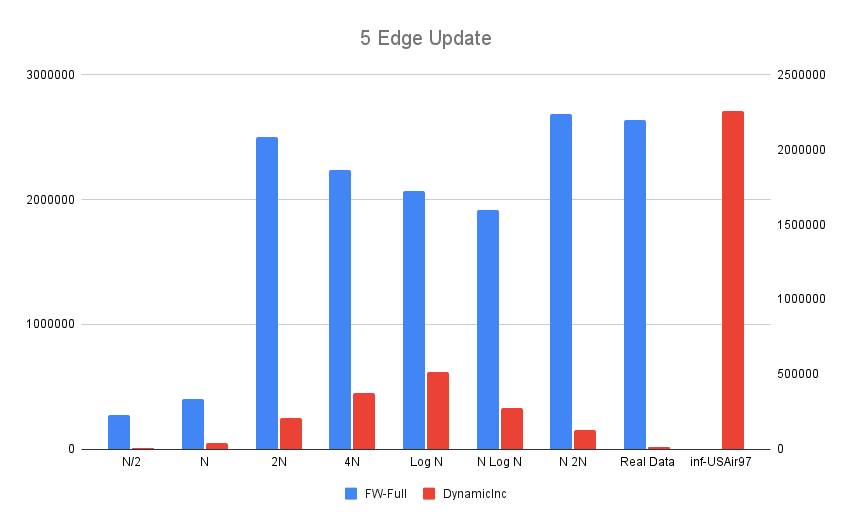
\includegraphics[width=8cm]{figures/5EdgeUpdate.png}
    \caption{Comparison of Floyd Warshall and DynamicInc for 5 updates}
    \label{fig:5edgeupdate}
\end{figure}

\begin{figure}[htp]
    \centering
    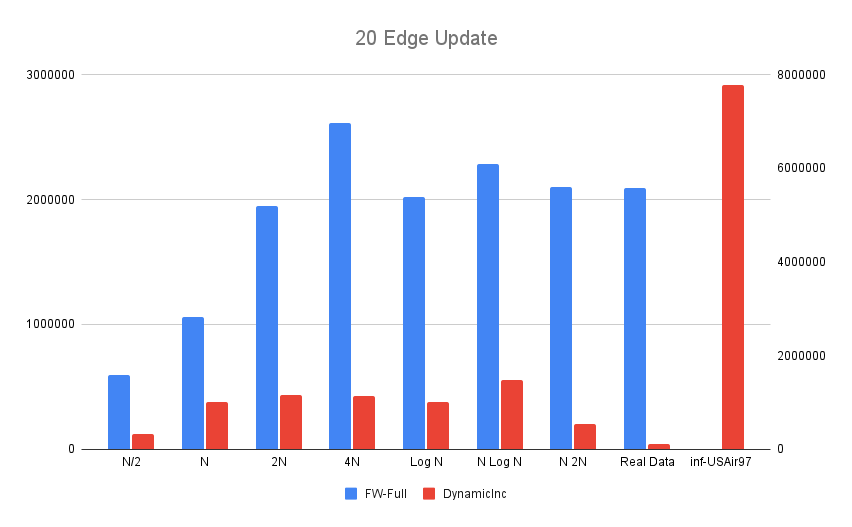
\includegraphics[width=8cm]{figures/20EdgeUpdate.png}
    \caption{Comparison of Floyd Warshall and DynamicInc for 20 updates}
    \label{fig:5edgeupdate}
\end{figure}

\begin{figure}[htp]
    \centering
    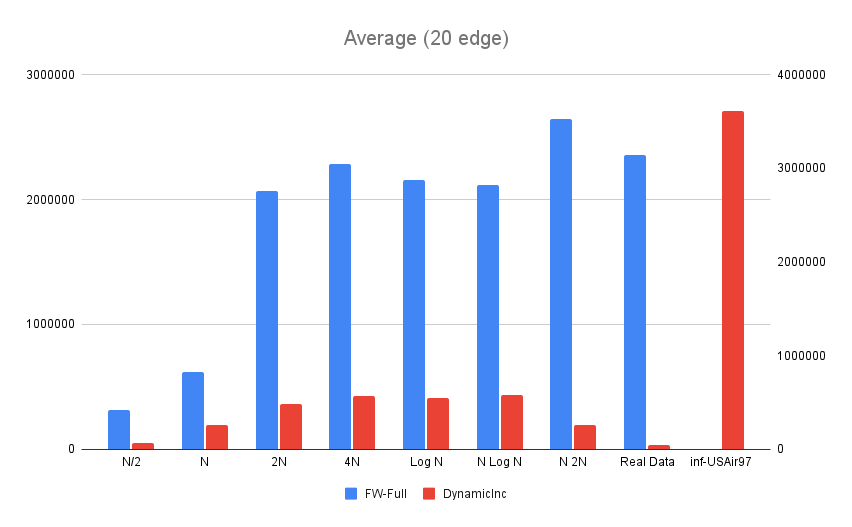
\includegraphics[width=8cm]{figures/Average.png}
    \caption{Comparison of Floyd Warshall and DynamicInc for Average of updates}
    \label{fig:5edgeupdate}
\end{figure}
\section{Conclusion}

Shortest Path computation is pivotal in real-world applications such as transportation networks where the graphs are dynamic in nature and can be used to calculate the shortest distance between each node especially in flight networks. In this paper, we have successfully presented a novel incremental algorithm for all pairs shortest path computations with the help of priority queues and using early stopping conditions over other algorithms such as QUINCA and RR. We achieved a significant improvement over naive methods and are able to get a better amortized complexity for node additions and edge updates in graph networks.

% \begin{itemize}
% \item Use either SI (MKS) or CGS as primary units. (SI units are encouraged.) English units may be used as secondary units (in parentheses). An exception would be the use of English units as identifiers in trade, such as ``3.5-inch disk drive''.
% \item Avoid combining SI and CGS units, such as current in amperes and magnetic field in oersteds. This often leads to confusion because equations do not balance dimensionally. If you must use mixed units, clearly state the units for each quantity that you use in an equation.
% \item Do not mix complete spellings and abbreviations of units: ``Wb/m\textsuperscript{2}'' or ``webers per square meter'', not ``webers/m\textsuperscript{2}''. Spell out units when they appear in text: ``. . . a few henries'', not ``. . . a few H''.
% \item Use a zero before decimal points: ``0.25'', not ``.25''. Use ``cm\textsuperscript{3}'', not ``cc''.)
% \end{itemize}

% \subsection{Equations}
% Number equations consecutively. To make your 
% equations more compact, you may use the solidus (~/~), the exp function, or 
% appropriate exponents. Italicize Roman symbols for quantities and variables, 
% but not Greek symbols. Use a long dash rather than a hyphen for a minus 
% sign. Punctuate equations with commas or periods when they are part of a 
% sentence, as in:
% \begin{equation}
% a+b=\gamma\label{eq}
% \end{equation}

% Be sure that the 
% symbols in your equation have been defined before or immediately following 
% the equation. Use ``\eqref{eq}'', not ``Eq.~\eqref{eq}'' or ``equation \eqref{eq}'', except at 
% the beginning of a sentence: ``Equation \eqref{eq} is . . .''

% \subsection{\LaTeX-Specific Advice}

% Please use ``soft'' (e.g., \verb|\eqref{Eq}|) cross references instead
% of ``hard'' references (e.g., \verb|(1)|). That will make it possible
% to combine sections, add equations, or change the order of figures or
% citations without having to go through the file line by line.

% Please don't use the \verb|{eqnarray}| equation environment. Use
% \verb|{align}| or \verb|{IEEEeqnarray}| instead. The \verb|{eqnarray}|
% environment leaves unsightly spaces around relation symbols.

% Please note that the \verb|{subequations}| environment in {\LaTeX}
% will increment the main equation counter even when there are no
% equation numbers displayed. If you forget that, you might write an
% article in which the equation numbers skip from (17) to (20), causing
% the copy editors to wonder if you've discovered a new method of
% counting.

% {\BibTeX} does not work by magic. It doesn't get the bibliographic
% data from thin air but from .bib files. If you use {\BibTeX} to produce a
% bibliography you must send the .bib files. 

% {\LaTeX} can't read your mind. If you assign the same label to a
% subsubsection and a table, you might find that Table I has been cross
% referenced as Table IV-B3. 

% {\LaTeX} does not have precognitive abilities. If you put a
% \verb|\label| command before the command that updates the counter it's
% supposed to be using, the label will pick up the last counter to be
% cross referenced instead. In particular, a \verb|\label| command
% should not go before the caption of a figure or a table.

% Do not use \verb|\nonumber| inside the \verb|{array}| environment. It
% will not stop equation numbers inside \verb|{array}| (there won't be
% any anyway) and it might stop a wanted equation number in the
% surrounding equation.

% \subsection{Some Common Mistakes}\label{SCM}
% \begin{itemize}
% \item The word ``data'' is plural, not singular.
% \item The subscript for the permeability of vacuum $\mu_{0}$, and other common scientific constants, is zero with subscript formatting, not a lowercase letter ``o''.
% \item In American English, commas, semicolons, periods, question and exclamation marks are located within quotation marks only when a complete thought or name is cited, such as a title or full quotation. When quotation marks are used, instead of a bold or italic typeface, to highlight a word or phrase, punctuation should appear outside of the quotation marks. A parenthetical phrase or statement at the end of a sentence is punctuated outside of the closing parenthesis (like this). (A parenthetical sentence is punctuated within the parentheses.)
% \item A graph within a graph is an ``inset'', not an ``insert''. The word alternatively is preferred to the word ``alternately'' (unless you really mean something that alternates).
% \item Do not use the word ``essentially'' to mean ``approximately'' or ``effectively''.
% \item In your paper title, if the words ``that uses'' can accurately replace the word ``using'', capitalize the ``u''; if not, keep using lower-cased.
% \item Be aware of the different meanings of the homophones ``affect'' and ``effect'', ``complement'' and ``compliment'', ``discreet'' and ``discrete'', ``principal'' and ``principle''.
% \item Do not confuse ``imply'' and ``infer''.
% \item The prefix ``non'' is not a word; it should be joined to the word it modifies, usually without a hyphen.
% \item There is no period after the ``et'' in the Latin abbreviation ``et al.''.
% \item The abbreviation ``i.e.'' means ``that is'', and the abbreviation ``e.g.'' means ``for example''.
% \end{itemize}
% An excellent style manual for science writers is \cite{b7}.

% \subsection{Authors and Affiliations}
% \textbf{The class file is designed for, but not limited to, six authors.} A 
% minimum of one author is required for all conference articles. Author names 
% should be listed starting from left to right and then moving down to the 
% next line. This is the author sequence that will be used in future citations 
% and by indexing services. Names should not be listed in columns nor group by 
% affiliation. Please keep your affiliations as succinct as possible (for 
% example, do not differentiate among departments of the same organization).

% \subsection{Identify the Headings}
% Headings, or heads, are organizational devices that guide the reader through 
% your paper. There are two types: component heads and text heads.

% Component heads identify the different components of your paper and are not 
% topically subordinate to each other. Examples include Acknowledgments and 
% References and, for these, the correct style to use is ``Heading 5''. Use 
% ``figure caption'' for your Figure captions, and ``table head'' for your 
% table title. Run-in heads, such as ``Abstract'', will require you to apply a 
% style (in this case, italic) in addition to the style provided by the drop 
% down menu to differentiate the head from the text.

% Text heads organize the topics on a relational, hierarchical basis. For 
% example, the paper title is the primary text head because all subsequent 
% material relates and elaborates on this one topic. If there are two or more 
% sub-topics, the next level head (uppercase Roman numerals) should be used 
% and, conversely, if there are not at least two sub-topics, then no subheads 
% should be introduced.

% \subsection{Figures and Tables}
% \paragraph{Positioning Figures and Tables} Place figures and tables at the top and 
% bottom of columns. Avoid placing them in the middle of columns. Large 
% figures and tables may span across both columns. Figure captions should be 
% below the figures; table heads should appear above the tables. Insert 
% figures and tables after they are cited in the text. Use the abbreviation 
% ``Fig.~\ref{fig}'', even at the beginning of a sentence.

% \begin{table}[htbp]
% \caption{Table Type Styles}
% \begin{center}
% \begin{tabular}{|c|c|c|c|}
% \hline
% \textbf{Table}&\multicolumn{3}{|c|}{\textbf{Table Column Head}} \\
% \cline{2-4} 
% \textbf{Head} & \textbf{\textit{Table column subhead}}& \textbf{\textit{Subhead}}& \textbf{\textit{Subhead}} \\
% \hline
% copy& More table copy$^{\mathrm{a}}$& &  \\
% \hline
% \multicolumn{4}{l}{$^{\mathrm{a}}$Sample of a Table footnote.}
% \end{tabular}
% \label{tab1}
% \end{center}
% \end{table}

% \begin{figure}[htbp]
% \centerline{
\includegraphics{fig1.png}}
% \caption{Example of a figure caption.}
% \label{fig}
% \end{figure}

% Figure Labels: Use 8 point Times New Roman for Figure labels. Use words 
% rather than symbols or abbreviations when writing Figure axis labels to 
% avoid confusing the reader. As an example, write the quantity 
% ``Magnetization'', or ``Magnetization, M'', not just ``M''. If including 
% units in the label, present them within parentheses. Do not label axes only 
% with units. In the example, write ``Magnetization (A/m)'' or ``Magnetization 
% \{A[m(1)]\}'', not just ``A/m''. Do not label axes with a ratio of 
% quantities and units. For example, write ``Temperature (K)'', not 
% ``Temperature/K''.

% \section{Experimentation}

% \section{Conclusion}

% \section*{Acknowledgment}

% The preferred spelling of the word ``acknowledgment'' in America is without 
% an ``e'' after the ``g''. Avoid the stilted expression ``one of us (R. B. 
% G.) thanks $\ldots$''. Instead, try ``R. B. G. thanks$\ldots$''. Put sponsor 
% acknowledgments in the unnumbered footnote on the first page.

% \section*{References}

% Please number citations consecutively within brackets \cite{b1}. The 
% sentence punctuation follows the bracket \cite{b2}. Refer simply to the reference 
% number, as in \cite{b3}---do not use ``Ref. \cite{b3}'' or ``reference \cite{b3}'' except at 
% the beginning of a sentence: ``Reference \cite{b3} was the first $\ldots$''

% Number footnotes separately in superscripts. Place the actual footnote at 
% the bottom of the column in which it was cited. Do not put footnotes in the 
% abstract or reference list. Use letters for table footnotes.

% Unless there are six authors or more give all authors' names; do not use 
% ``et al.''. Papers that have not been published, even if they have been 
% submitted for publication, should be cited as ``unpublished'' \cite{b4}. Papers 
% that have been accepted for publication should be cited as ``in press'' \cite{b5}. 
% Capitalize only the first word in a paper title, except for proper nouns and 
% element symbols.

% For papers published in translation journals, please give the English 
% citation first, followed by the original foreign-language citation \cite{b6}.



\bibliographystyle{IEEEtran}
\bibliography{ref}

\appendix
\begin{algorithm}[H]
\caption{IncrementalInsertNode}
\begin{algorithmic}[1]
\Require A $graph$ represented with:
\begin{itemize}
    \item $dist$: A 2D list containing distances between nodes.
    \item $predecessors$: A 2D list showing the predecessor of each node.
\end{itemize}
\Require A new node $z$, and its distances:
\begin{itemize}
    \item $z_{in}$: List of distances from $z$ to other nodes.
    \item $z_{out}$: List of distances from other nodes to $z$.
\end{itemize}
\State Extend $dist$ and $predecessors$ to accommodate the new node.
\For{$i = 0$ to $graph.numNodes$}
    \State $dist[z][i] \leftarrow z_{out}[i]$
    \State $dist[i][z] \leftarrow z_{in}[i]$
    \If{$z_{out}[i] < \infty$}
        \State $predecessors[z][i] \leftarrow z$
    \EndIf
    \If{$z_{in}[i] < \infty$}
        \State $predecessors[i][z] \leftarrow i$
    \EndIf
\EndFor
\State Initialize a priority queue $pq$
\State $pq.push((0, z))$
\While{not $pq.empty()$}
    \State $(d, u) \leftarrow pq.pop()$
    \For{$v = 0$ to $graph.numNodes$}
        \If{$dist[u][v] < \infty$}
            \State $new\_dist \leftarrow d + dist[u][v]$
            \If{$new\_dist < dist[z][v]$}
                \State $dist[z][v] \leftarrow new\_dist$
                \State $predecessors[z][v] \leftarrow u$
                \State $pq.push((new\_dist, v))$
            \EndIf
        \EndIf
    \EndFor
    \For{$i = 0$ to $graph.numNodes$}
        \For{$j = 0$ to $graph.numNodes$}
            \If{$dist[i][z] + dist[z][j] < dist[i][j]$}
                \State $dist[i][j] \leftarrow dist[i][z] + dist[z][j]$
                \State $predecessors[i][j] \leftarrow predecessors[z][j]$
            \EndIf
        \EndFor
    \EndFor
\EndWhile
\end{algorithmic}
\end{algorithm}





\end{document}
